\begin{frame}{Fragestellung}
  \begin{columns}
    \begin{column}{0.5\textwidth}
      \begin{block}{Definition}
        \begin{itemize}
          \item Klassifikation von Himmelfotos in 9 Wolkenklassen
        \end{itemize}
      \end{block}
      \begin{block}{Motivation}
        \begin{itemize}
          \item Wettervorhersage mit primitiven Mitteln
            \begin{itemize}
              \item[$\supset$] \alert{Wolkenklassifikation}
            \end{itemize}
        \end{itemize}
      \end{block}
    \end{column}
    \begin{column}{0.5\textwidth}
      \centering
      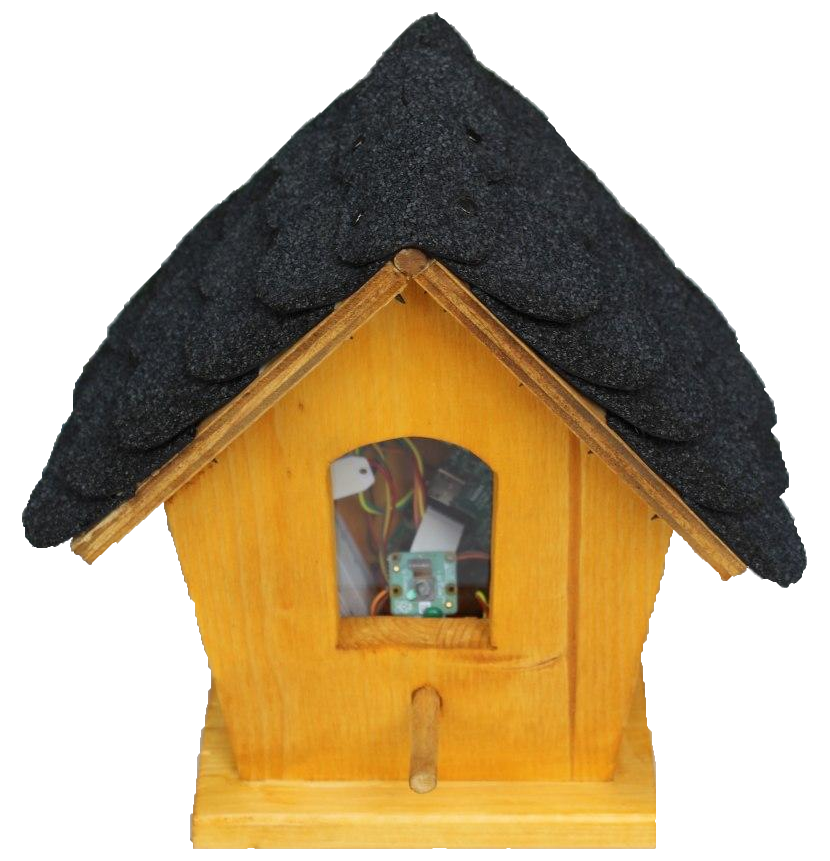
\includegraphics[height=0.7\textheight]{content/wetterstation.png}
    \end{column}
  \end{columns}
\end{frame}

\begin{frame}{Datensatz}
  \begin{columns}
    \begin{column}{0.5\textwidth}
      \begin{itemize}
        \item \# Fotos $> \SI{10}{\hour\per\day} \cdot \SI{4}{\per\hour} \cdot \si{\day}$
        \item $1024 \times 768$ Pixel
      \end{itemize}
    \end{column}
    \begin{column}{0.5\textwidth}
      \centering
      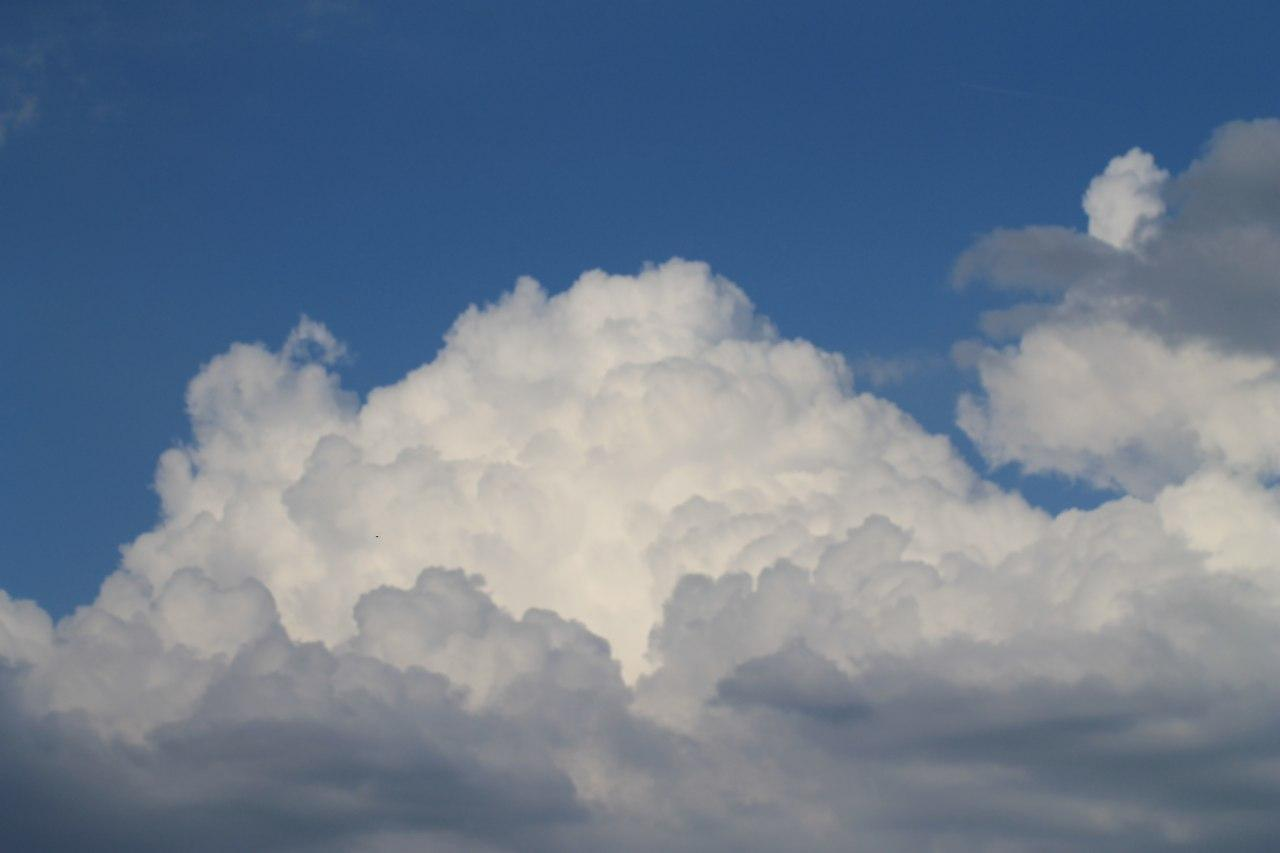
\includegraphics[width=\textwidth]{content/wolke01.jpg}
    \end{column}
  \end{columns}
\end{frame}

\begin{frame}{Alternativmethoden}
  \begin{enumerate}
    \item Random Forest auf Farbspektrum
    \item kNN auf Mean-Bild oder gebauten Features der jeweiligen Klasse
    \item[\Rightarrow] Vergleiche Genauigkeit, Laufzeit, Robustheit
  \end{enumerate}
\end{frame}
